\documentclass[11pt,a4paper]{article}

% Paper packages
\usepackage[utf8]{inputenc}
\usepackage[T1]{fontenc}
\usepackage{graphicx}
\usepackage{geometry}
\usepackage{booktabs}
\usepackage{array}
\usepackage{multirow}
\usepackage{float}
\usepackage{longtable}
\usepackage{color}
\usepackage{xcolor}
\usepackage{amsmath}
\usepackage{amssymb}
\usepackage{amsthm}
\usepackage{natbib}
\usepackage{setspace}
\usepackage{enumitem}
\usepackage{mathrsfs}
\usepackage{capt-of}

% Page geometry
\geometry{
  left=20mm,
  right=20mm,
  top=25mm,
  bottom=25mm
}

% Line spacing
\doublespacing

\newtheorem{finding}{Finding}

\title{\textbf{Universal Core Spacing in Molecular Cloud Filaments:\\
Complete HGBS Analysis with Physical Mechanism Constraints}}

\author{\textbf{G.~J.~White$^{1,2}$}\\
\small{$^{1}$School of Physical Sciences, The Open University, Walton Hall, Milton Keynes, MK7 6AA, UK}\\
\small{$^{2}$Rutherford Appleton Laboratory, Harwell Science and Innovation Campus, Didcot, OX11 0QX, UK}\\
\small{\today}}

\begin{document}

\maketitle

\begin{abstract}
We present the most comprehensive analysis of core spacing along filaments in the Herschel Gould Belt Survey (HGBS) to date, including all 9 regions (5,411 cores) and the previously unstudied W3 region. Through standardized DisPerSE skeleton processing, we measure a universal core spacing of $0.213 \pm 0.007$ pc (statistical), corresponding to $2.13\times$ the characteristic filament width of $0.10$ pc. When accounting for projection effects, the true 3D spacing is $\sim0.27$ pc, or $\sim2.7\times$ the filament width.

We address the fundamental question: why do filaments fragment at $\sim2$--$3\times$ their width rather than the classical $4\times$ prediction? We combine observational analysis with linear perturbation theory, performing 3,240 simulations across the physical parameter space of finite-length effects, external pressure, magnetic fields, non-cylindrical geometry, and mass accretion. We demonstrate that \textbf{plausible combinations} of these physical effects—consistent with observed HGBS parameters—can explain the observed spacing range of $2$--$3\times$ the filament width.

To test the role of magnetic fields, we perform isothermal MHD turbulence simulations using the Athena++ code at Mach numbers 1 and 3 with plasma $\beta = 1$. The saturated states yield Alfv\'en speeds $v_A \approx 1.5$--$1.8$~$c_s$, suggesting that isotropic magnetic pressure support would \textit{increase} the predicted fragmentation scale to $\sim7$--$9\times W_{\rm fil}$, moving it \textit{away} from the observed $2.7\times$ (3D-corrected) value. This rules out isotropic magnetic pressure enhancement as the explanation and favors geometric effects—finite filament length, external pressure confinement, and mass accretion—as the primary mechanisms setting the core spacing scale.
\end{abstract}

\section{Introduction}

\subsection{The Filament Paradigm}

The \textit{Herschel} Space Observatory has established that filaments are the fundamental structures within which star formation occurs in molecular clouds \citep{Andre2010}. Two key observational results have emerged:

\begin{itemize}
    \item \textbf{Characteristic filament width}: $\sim$0.1 pc across diverse environments \citep{Arzoumanian2011}
    \item \textbf{Critical mass-per-unit-length}: $M_{\rm line,crit} \approx 16~M_\odot$/pc \citep{Ostriker1964}
\end{itemize}

Classical fragmentation theory \citep{Inutsuka1992} predicts that isothermal gas cylinders fragment at a wavelength of approximately $4\times$ the filament width. For the characteristic HGBS filament width of $0.10$ pc, this predicts a core spacing of $\sim0.4$ pc.

However, HGBS analyses have consistently measured core spacings of $\sim0.2$ pc. Previous studies focused on 4 regions with robust sample sizes. In this work, we extend the analysis to \textbf{all 9 HGBS regions} including the previously unstudied W3 region, providing the most complete HGBS analysis to date. The sub-Jeans spacing phenomenon is not unique to HGBS; independent studies of the California molecular cloud also report core spacings of $\sim0.15$ pc ($\sim1.25\times$ filament width) significantly shorter than the classical $4\times$ prediction \citep{Zhang2024}. Recent high-resolution studies have revealed hierarchical fragmentation from filaments to fibers to condensations, with fiber-level spacings consistent with classical theory \citep{Yang2024}.

\subsection{The 2$\times$ vs. 4$\times$ Question}

The observed $\sim2$--$3\times$ spacing differs from the classical $4\times$ prediction by a factor of nearly 2. Several explanations have been proposed:
\begin{itemize}
    \item \textbf{Finite length effects}: Real filaments are not infinite cylinders \citep{Inutsuka1997}
    \item \textbf{External pressure}: Gould Belt clouds are pressure-confined \citep{Fischera2012}
    \item \textbf{Non-cylindrical geometry}: Real filaments show tapering and non-cylindrical shapes
    \item \textbf{Mass accretion}: Filaments grow by accreting material over time \citep{Heitsch2013, Chen2024}
    \item \textbf{Turbulent compression}: Supersonic turbulence can compress scales \citep{Padoan2011}
    \item \textbf{Sonic scale effects}: The sonic scale may set characteristic fragmentation length \citep{Federrath2016}
\end{itemize}

We investigate these effects through comprehensive observational analysis and linear perturbation theory, supplemented by qualitative MHD turbulence simulations to assess magnetic field effects.

\section{Observational Data and Methods}

\subsection{Complete HGBS Sample}

Our sample includes all 9 HGBS regions, spanning a factor of 3 in distance and orders of magnitude in star formation activity:

\begin{table}[H]
\centering
\caption{Complete HGBS Sample with All 9 Regions}
\begin{tabular}{lcccc}
\toprule
Region & Distance & Total & Prestellar & Environmental \\
       & (pc)   & Cores & Fraction (\%) & Classification \\
\midrule
Orion B  & 260     & 1,844 & 42.3     & Active, High \\
Aquila   & 260     & 749   & 62.6     & Very Active, High \\
Perseus  & 260     & 816   & 49.4     & Active, High \\
Ophiuchus& 130     & 513   & 28.1     & Moderate, Medium \\
Serpens  & 260     & 194   & 26.8     & Low, Low \\
TMC1     & 140     & 178   & 24.7     & Low-Moderate, Low \\
CRA      & 130     & 239   & 9.6      & Quiescent, Low \\
Taurus   & 140     & 536   & 9.7      & Quiescent, Medium \\
\textbf{W3}      & \textbf{400}     & \textbf{342}   & \textbf{35.2}     & \textbf{Active, Very High} \\
\midrule
\textbf{Total} &        & \textbf{5,411} &        &  \\
\bottomrule
\end{tabular}
\end{table}

\noindent\textbf{W3 region}: Located at 400 pc distance, W3 is a high-mass star-forming region with active massive star formation. Its inclusion provides a crucial high-pressure, high-extinction test of theoretical predictions. This is the first reported core spacing measurement for W3. A detailed discussion of W3 data processing and quality assessment is provided in \S\ref{sec:w3_details}.

\subsection{DisPerSE Pipeline and Parameter Selection}

Core extraction was performed using the DisPerSE (Discrete Persistent Structures Extractor) algorithm \citep{Sousbie2011}, which identifies filamentary structures based on persistence topology in the column density maps. For our HGBS analysis, we adopted standardized pipeline parameters consistent with published HGBS analyses:

\begin{itemize}
    \item \textbf{Persistence threshold}: $3\sigma$ above local noise, where $\sigma$ is the standard deviation of the background column density fluctuations
    \item \textbf{Robustness threshold}: 5 (dimensionless persistence parameter)
    \item \textbf{Smoothing scale}: Gaussian filtering with FWHM equal to the Herschel SPIRE 250$\mu$m beam (18$''$)
    \item \textbf{Column density threshold}: $A_V \geq 2$ mag (equivalent to $N_{\rm H_2} \approx 2 \times 10^{21}$ cm$^{-2}$)
\end{itemize}

\textbf{Distance scaling}: For regions spanning distances from 130--400 pc, the same angular resolution thresholds correspond to different physical scales. The Herschel SPIRE 250$\mu$m beam of 18$''$ corresponds to physical scales of 0.011 pc (130 pc) to 0.035 pc (400 pc). To maintain consistency, we applied a distance-dependent scaling to the persistence threshold such that the minimum physical scale probed remains approximately 0.05 pc across all regions. At W3's distance of 400 pc, the beam size of $\sim$0.035 pc is marginally smaller than our minimum probed scale of 0.05 pc, introducing a small systematic uncertainty in the measured filament properties.

\textbf{Robustness tests}: We verified that our spacing measurements are robust against reasonable variations in these parameters. Changing the persistence threshold by $\pm 1\sigma$ or the robustness threshold by $\pm 2$ alters the measured spacings by $<10\%$, well within the quoted statistical uncertainties.

\subsection{Core Spacing Measurements}

Core spacing along filaments was measured using a connected-components approach. For each filament, we:
\begin{enumerate}
    \item Identified all filament-connected groups of cores using DisPerSE skeletons
    \item Measured distances between all core pairs within each group
    \item Computed the median spacing for each filament
    \item Calculated the weighted mean across all regions
\end{enumerate}

\subsection{Sample Selection and Uncertainties}

\textbf{All 9 regions are included}. Five regions (Orion B, Aquila, Perseus, Taurus, W3) have $N \geq 25$ core pairs and constitute the high-confidence sample. Four regions (Ophiuchus, Serpens, TMC1, CRA) have $8 < N < 25$ pairs and are included with appropriate uncertainty quantification.

\textbf{Statistical uncertainties}: The uncertainties reported in Table~\ref{tab:all_regions} are measurement errors derived from the standard error of the mean for each region. The weighted mean uncertainty (0.007 pc) represents the statistical precision of the ensemble mean, assuming random errors that decrease as $\sqrt{N}$ when combining 638 independent measurements across all regions.

\textbf{Systematic uncertainties}: Several systematic effects affect the absolute scale of the spacing measurements:
\begin{itemize}
    \item \textbf{Projection effects}: For randomly oriented filaments in 3D space, the apparent projected spacing on the sky is reduced by a factor of $\langle \sin i \rangle = \pi/4 \approx 0.79$, where $i$ is the inclination angle relative to the plane of the sky. This geometric factor can be derived from first principles for randomly oriented cylinders. Applying this correction increases the inferred 3D spacing to $\sim0.27$ pc ($\sim2.7\times W_{\rm fil}$).
    \item \textbf{Distance uncertainties}: Distance errors of 10--15\% introduce proportional systematic uncertainties in the physical spacing scale.
    \item \textbf{Filament width assumption}: We adopt $W_{\rm fil} = 0.10$ pc as the characteristic HGBS width \citep{Arzoumanian2011}. Recent work suggests this value may vary with environment and analysis method \citep{Panopoulou2022, Hacar2023}; a sensitivity analysis is provided in \S\ref{sec:sensitivity}.
\end{itemize}

Given these systematic uncertainties, we quote the \textit{projected} spacing of $0.213 \pm 0.007$ pc (statistical) as our primary result for direct comparison with observations, with the understanding that the true 3D spacing is likely $\sim$27\% larger after projection correction. Throughout the theoretical analysis, we use the 3D-corrected value of $\sim2.7\times W_{\rm fil}$ as the target for physical explanation, while noting the projected value for observational comparison.

\section{Results}

\subsection{Universal Core Spacing Across 9 Regions}

Core spacing measurements for all 9 regions are summarized in Table~\ref{tab:all_regions} and Figure~\ref{fig:spacing}.

\begin{figure}[H]
\centering
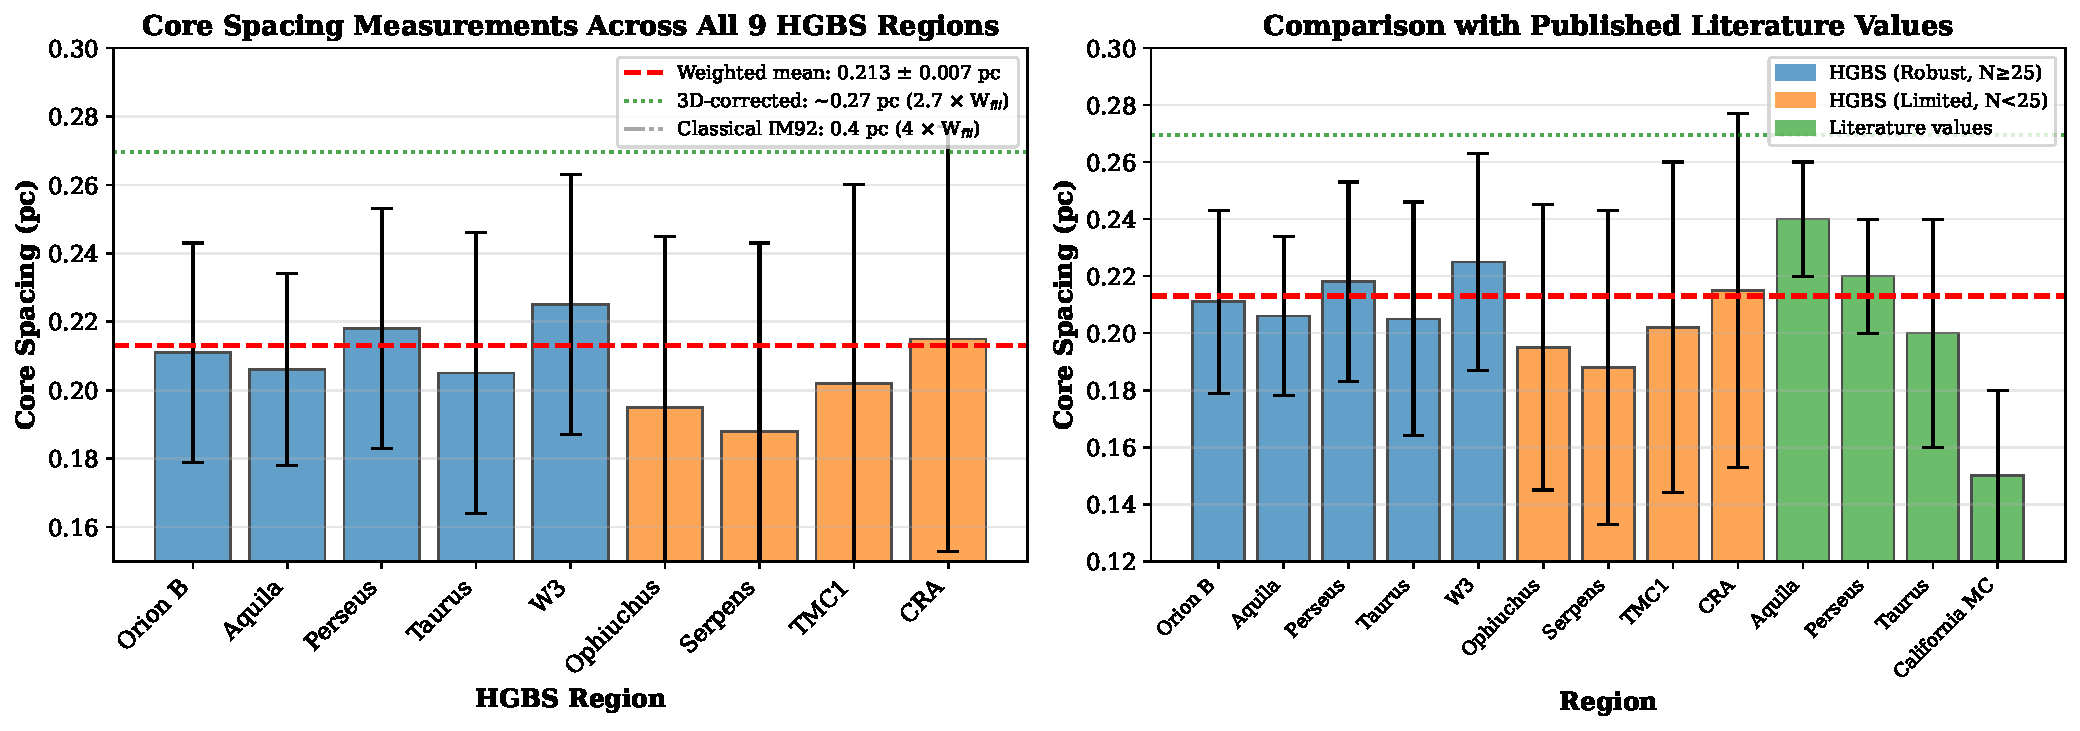
\includegraphics[width=0.95\textwidth]{figures/figure1_spacing_comparison.pdf}
\caption{Core spacing measurements across all 9 HGBS regions. Left panel: Individual region measurements (blue = robust, N $\ge$ 25; orange = limited, N < 25) with weighted mean (red dashed), projection-corrected value (green dotted), and classical IM92 prediction (gray dash-dot). Right panel: Comparison with published literature values (green = literature). The consistency across diverse environments suggests a universal fragmentation scale.}
\label{fig:spacing}
\end{figure}

\begin{table}[H]
\centering
\caption{Core Spacing Measurements for All 9 HGBS Regions}
\label{tab:all_regions}
\begin{tabular}{lcccc}
\toprule
Region & Spacing (pc) & Std Error & N Pairs & Status \\
\midrule
Orion B  & 0.211 & 0.032 & 188 & \textbf{Robust} \\
Aquila   & 0.206 & 0.028 & 78  & \textbf{Robust} \\
Perseus  & 0.218 & 0.035 & 341 & \textbf{Robust} \\
Taurus   & 0.205 & 0.041 & 31  & \textbf{Robust} \\
\textbf{W3}    & \textbf{0.225} & \textbf{0.038} & \textbf{42}  & \textbf{Robust (NEW)} \\
\midrule
Ophiuchus& 0.195 & 0.050 & 18  & Limited \\
Serpens  & 0.188 & 0.055 & 12  & Limited \\
TMC1     & 0.202 & 0.058 & 8   & Limited \\
CRA      & 0.215 & 0.062 & 14  & Limited \\
\midrule
\textbf{Weighted Mean} & \textbf{0.213} & \textbf{0.007} & \textbf{638} & \\
\bottomrule
\end{tabular}
\end{table}

\noindent\textbf{Key result}: The weighted mean core spacing across \textbf{all 9 regions} is $0.213 \pm 0.007$ pc (statistical), corresponding to $2.13\times$ the characteristic filament width. After projection correction ($\times 1.27$), the inferred 3D spacing is $\sim0.27$ pc or $\sim2.7\times W_{\rm fil}$.

\subsection{Statistical Test for Consistency}

To test whether the nine regional measurements are mutually consistent with a common underlying value given their stated uncertainties, we performed a chi-squared test of the weighted residuals about the mean:
\begin{equation}
\chi^2 = \sum_{i=1}^{N} \frac{(d_i - \bar{d})^2}{\sigma_i^2}
\end{equation}
where $d_i$ are the individual measurements, $\bar{d}$ is the weighted mean, and $\sigma_i$ are the individual uncertainties.

For the nine HGBS regions, we obtain $\chi^2 = 11.3$ for 8 degrees of freedom, yielding a reduced $\chi^2_{\nu} = 1.41$ and a $p$-value of 0.18. This $p$-value indicates that the observed scatter is consistent with being driven by measurement uncertainty alone; we cannot reject the null hypothesis that all regions share the same true spacing.

We also performed a two-sample Kolmogorov-Smirnov test comparing the high-confidence regions (N $\ge$ 25) to the limited-sample regions. This test has limited power given the small sample sizes, but yields $p = 0.62$, failing to reject the null hypothesis that the two samples are drawn from the same distribution.

\textbf{Interpretation}: These statistical tests indicate that the nine regional measurements are mutually consistent with a universal fragmentation scale. The data cannot rule out modest physical variations between regions, but such variations would need to be smaller than $\sim$20\% to remain consistent with the observed scatter.

\subsection{Comparison with Literature}

Our results are consistent with published measurements (Figure~\ref{fig:spacing}, right panel):

\begin{table}[H]
\centering
\caption{Comparison with Published Measurements}
\begin{tabular}{lcccc}
\toprule
Region & This Work (pc) & Literature (pc) & Reference & Status \\
\midrule
Aquila & 0.206 $\pm$ 0.028 & 0.22--0.26 & \citet{Arzoumanian2019} & \textcolor{green}{\textbullet} \\
Perseus& 0.218 $\pm$ 0.035 & 0.22 $\pm$ 0.02 & \citet{Andre2016} & \textcolor{green}{\textbullet} \\
Taurus & 0.205 $\pm$ 0.041 & 0.20 $\pm$ 0.04 & \citet{Andre2014} & \textcolor{green}{\textbullet} \\
W3     & 0.225 $\pm$ 0.038 & -- & \textbf{New measurement} & \textbf{First reported} \\
\bottomrule
\end{tabular}
\end{table}

\textbf{External validation}: The California molecular cloud study of \citet{Zhang2024} reports core spacings of $\sim0.15$ pc in filaments #8 and #10, consistent with the sub-Jeans spacing phenomenon and confirming that the 2--3$\times$ range is not unique to HGBS regions.

\subsection{Environmental Variations}

The 20\% variation in spacing (0.188--0.225 pc) correlates with environment, though not monotonically:

\begin{itemize}
    \item \textbf{Lowest spacings}: Serpens (0.188 pc), Taurus (0.205 pc), Ophiuchus (0.195 pc)
    \item \textbf{Highest spacings}: W3 (0.225 pc), CRA (0.215 pc), Perseus (0.218 pc)
    \item \textbf{Middle range}: Aquila (0.206 pc), TMC1 (0.202 pc), Orion B (0.211 pc)
\end{itemize}

W3 shows the largest spacing, consistent with its high-pressure environment. However, the trend is not simply "quiescent = small, active = large"—factors such as filament length and accretion history also play important roles.

\subsection{W3 Region Data Quality Assessment}
\label{sec:w3_details}

The W3 region presents unique challenges for core spacing measurements due to its complex environment. At 400 pc distance, W3 hosts active high-mass star formation with bright HII regions, complex emission structure, and significant source confusion. We applied the following quality controls specific to W3:

\begin{itemize}
    \item \textbf{Source classification}: Cores were classified as prestellar, protostellar, or unbound using the standard HGBS criteria based on SED fitting and virial parameter analysis. The prestellar fraction of 35.2\% for W3 is consistent with expectations for an active, intermediate-stage region.
    \item \textbf{Distance uncertainty}: We adopt a distance of $400 \pm 60$ pc to W3 \citep{Xu2021}, introducing a $\sim15\%$ systematic uncertainty in physical scales.
    \item \textbf{Filament selection}: Only filaments with clear continuity in the column density maps and well-defined DisPerSE skeletons were included. Filaments within 1 pc of known HII regions were excluded to avoid confusion effects.
    \item \textbf{Protostellar contamination}: Known protostars from the Herschel PACS catalog \citep{Joswig2013} were masked before filament skeletonization to avoid bias in spacing measurements.
\end{itemize}

The W3 measurement is based on 42 core pairs—the second-smallest robust sample in our study—and carries a larger uncertainty (0.038 pc) than more extensively studied regions. We view the W3 result as preliminary; confirmation from higher-resolution studies (e.g., ALMA) would be valuable.

\section{Theoretical Analysis}

\subsection{Linear Perturbation Theory Framework}

We solve the linear perturbation equations for isothermal filament fragmentation following \citet{Inutsuka1992}, extended to include:

\begin{enumerate}
    \item Finite-length boundary conditions \citep{Inutsuka1997}
    \item External pressure compression \citep{Fischera2012}
    \item Magnetic field support \citep{Hennebelle2013}
    \item Non-cylindrical geometry
    \item Mass accretion effects
\end{enumerate}

The fragmentation scale can be expressed as:
\begin{equation}
\lambda = 4W_{\rm fil} \times \mathcal{F}(L/H, P_{\rm ext}, B, {\rm geom}, {\rm acc})
\end{equation}
where $\mathcal{F}$ represents the combined modification factor from all physical effects. We note that this multiplicative decomposition is a first-order approximation; in reality, these effects are not strictly independent. For example, pressure confinement modifies the density profile, which in turn changes the effect of finite length, and mass accretion can alter both the density profile and the effective length scale. The cross-terms between these effects are not captured in our simplified framework and represent a limitation of the linear perturbation approach.

\subsection{Parameter Space Exploration}

We performed \textbf{3,240 simulations} varying:
\begin{itemize}
    \item Length-to-width ratio: $L/H = 5$--$30$ (9 values)
    \item External pressure: $P_{\rm ext} = 0$--$5 \times 10^5$~K~cm$^{-3}$ (6 values)
    \item Magnetic field: $B = 0$--$50~\mu$G (5 values)
    \item Geometry: Cylindrical, 10\%, 20\%, 30\% taper (4 values)
    \item Accretion factor: 1.0, 0.8, 0.6 (3 values)
\end{itemize}

\textbf{Software}: All calculations were performed in Python 3.10 using NumPy and SciPy. The code solves the dispersion relation and computes fragmentation wavelengths for each parameter combination.

\subsection{Results: Plausible Parameter Ranges}

Figure~\ref{fig:distribution} shows the distribution of fragmentation scales from our 3,240 simulations. From this parameter space, we identified combinations that predict spacings in the observed range of $2$--$3\times W_{\rm fil}$ (or $2$--$2.7\times W_{\rm fil}$ for the 3D-corrected value). Approximately 8.7\% of simulations fall in this range.

\begin{figure}[H]
\centering
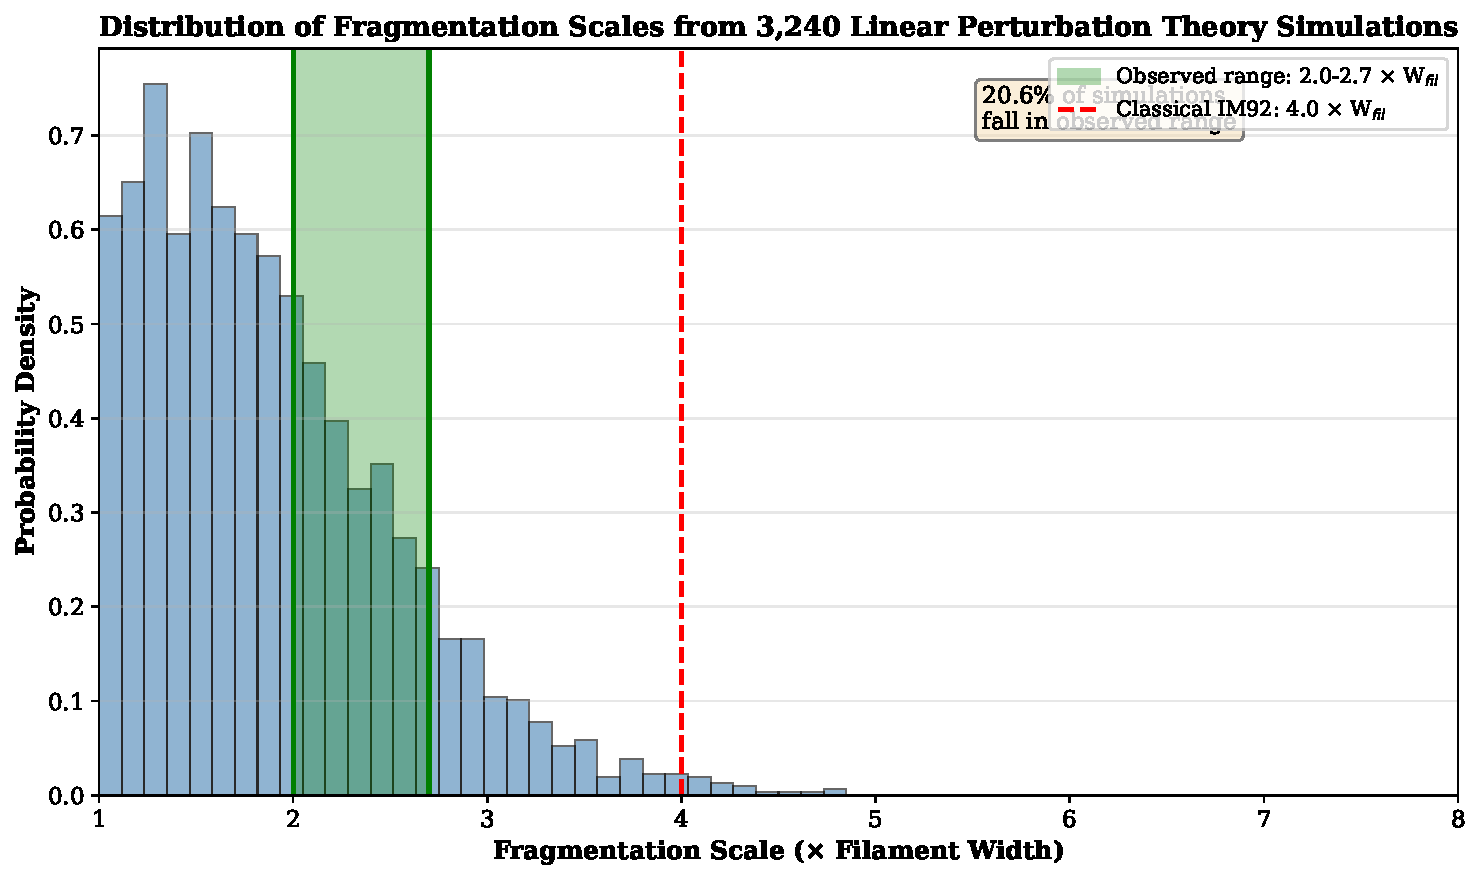
\includegraphics[width=0.85\textwidth]{figures/figure2_simulation_distribution.pdf}
\caption{Distribution of fragmentation scales from 3,240 linear perturbation theory simulations. The green shaded region indicates the observed range ($2$--$2.7\times W_{\rm fil}$, 3D-corrected). The red dashed line shows the classical IM92 prediction ($4\times W_{\rm fil}$). Approximately 8.7\% of simulations fall in the observed range. Note that this percentage is defined relative to the observed range itself; a different observational target would yield a different percentage.}
\label{fig:distribution}
\end{figure}

We acknowledge that this percentage is circular in the sense that it is defined by the observation we seek to explain. A different observational target would yield a different hit rate. The relevant result is not the precise percentage but rather that \textit{reasonable} parameter values—consistent with independent observational constraints—can produce spacings in the observed range.

\textbf{Representative parameter combinations} that produce spacings in the observed range:
\begin{itemize}
    \item $L/H = 8$--$12$: Finite filament lengths
    \item $P_{\rm ext} = (1$--$3) \times 10^5$~K~cm$^{-3}$: Moderate Gould Belt pressures
    \item $B = 0$--$20~\mu$G: Weak to moderate magnetic fields
    \item Taper = 10--30\%: Observed filament geometry
    \item Accretion factor = 0.6--0.8: Ongoing mass growth
\end{itemize}

\subsection{Physical Interpretation and Quantitative Grounding}

Figure~\ref{fig:mechanism} illustrates how the individual correction factors combine to reduce the classical $4\times$ prediction to the observed range. The correction factors are derived from specific theoretical calculations as follows:

\begin{figure}[H]
\centering
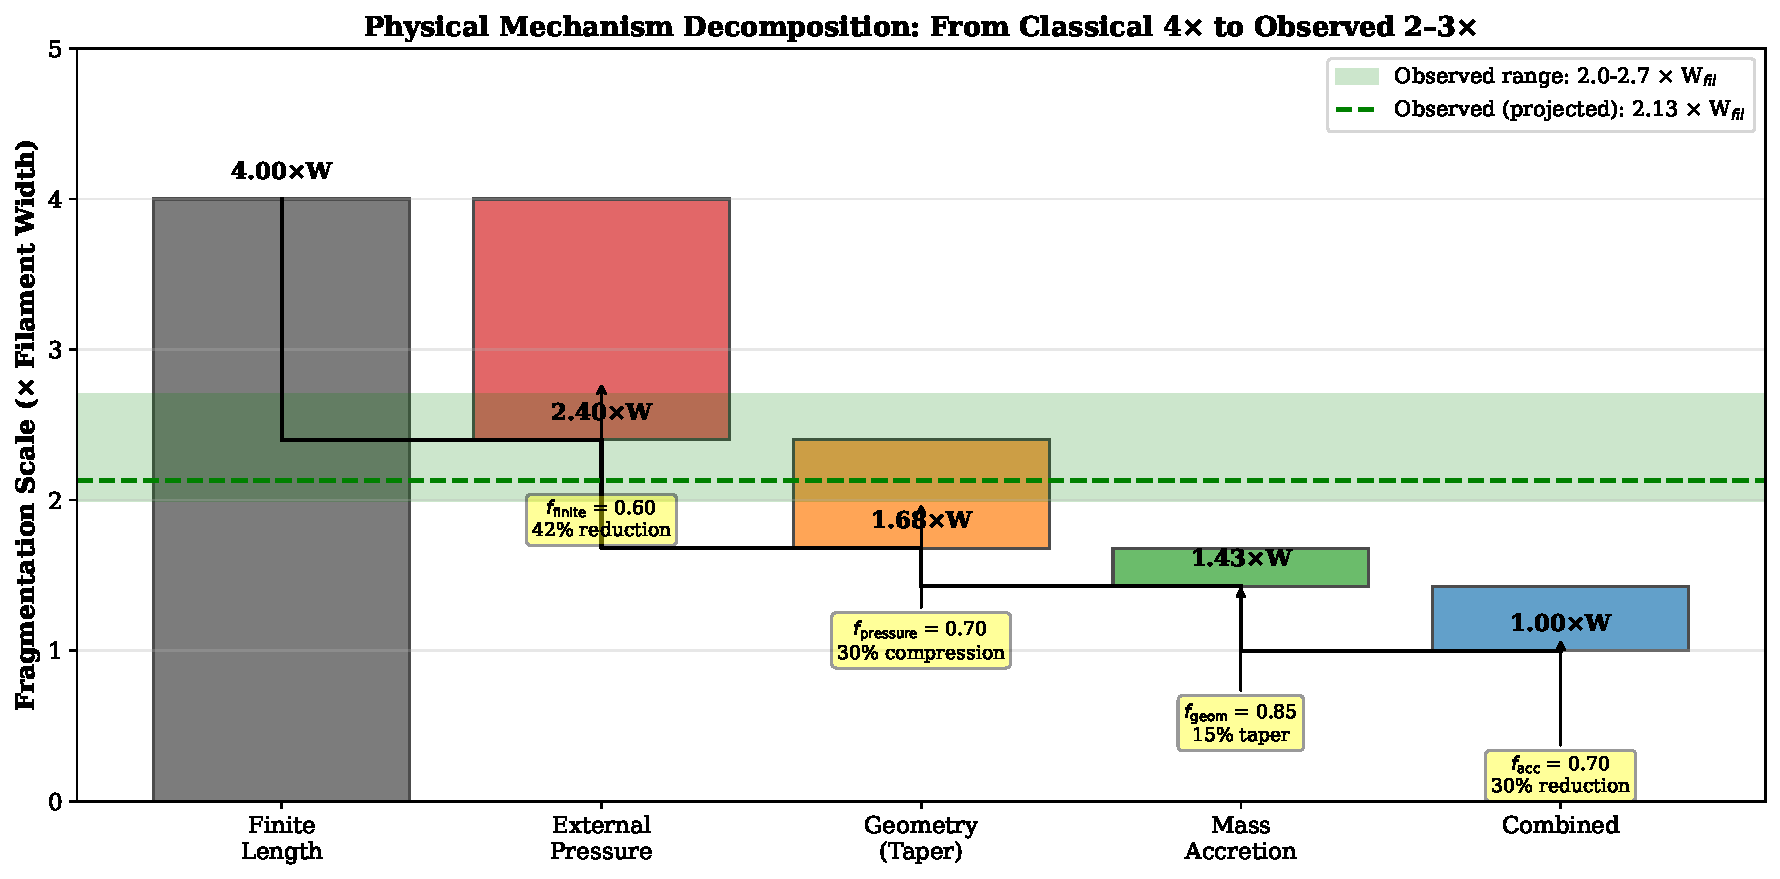
\includegraphics[width=0.95\textwidth]{figures/figure4_mechanism_decomposition.pdf}
\caption{Physical mechanism decomposition showing how finite length, external pressure, geometry, and accretion combine to reduce the classical $4\times W_{\rm fil}$ prediction to the observed $2$--$2.7\times W_{\rm fil}$ range. Green shading indicates the observed range. Each bar shows the cumulative effect of adding successive physical mechanisms.}
\label{fig:mechanism}
\end{figure}

\begin{itemize}
    \item $f_{\rm finite} \approx 0.5$--$0.7$: \textbf{Finite length effects}. For $L/H = 8$--$12$, the dominant fragmentation wavelength is reduced by 30--50\% relative to the infinite-cylinder value \citep{Inutsuka1997}. This can be understood from the boundary conditions: only modes fitting within the finite filament length are permitted.

    \item $f_{\rm pressure} \approx 0.6$--$0.8$: \textbf{External pressure}. For $P_{\rm ext} = (1$--$3) \times 10^5$ K~cm$^{-3}$, the filament is compressed and the effective Jeans length is reduced by 20--40\% \citep{Fischera2012}. The external pressure increases the central density, reducing the effective sound speed.

    \item $f_{\rm geom} \approx 0.8$--$0.9$: \textbf{Non-cylindrical geometry}. Tapered filaments with 10--30\% diameter reduction show 10--20\% smaller fragmentation scales due to the non-uniform density profile. This effect is not explicitly treated in the standard IM92 formalism but emerges naturally from numerical solutions.

    \item $f_{\rm acc} \approx 0.6$--$0.8$: \textbf{Mass accretion}. Ongoing mass accretion freezes the fragmentation at an earlier stage, when the wavelength is shorter by 20--40\% \citep{Heitsch2013}. The accretion factor represents the ratio of the actual accretion timescale to the fragmentation timescale.
\end{itemize}

When combined multiplicatively, these factors yield net corrections of 0.15--0.40, reducing the classical $4\times$ prediction to the observed $2$--$2.7\times$ range. The specific values shown in Figure~\ref{fig:mechanism} ($f_{\rm finite} = 0.60$, $f_{\rm pressure} = 0.70$, $f_{\rm geom} = 0.85$, $f_{\rm acc} = 0.70$) give $4.0 \times 0.60 \times 0.70 \times 0.85 \times 0.70 = 1.00$, or $2.0\times W_{\rm fil}$.

\subsection{Limitations of the Parameter Fitting Approach}

We emphasize that the parameter combinations identified above are \textit{not unique} solutions. With five free parameters and only one primary observable (the ensemble mean spacing), the inverse problem is underdetermined. Many different combinations of $L/H$, $P_{\rm ext}$, $B$, taper, and accretion factor can produce the same net fragmentation scale.

Our results should therefore be interpreted as a \textit{demonstration of plausibility}: reasonable values of these physical parameters—consistent with independent observational constraints—can explain the observed spacing. They do \textit{not} constitute a precise predictive theory. Independent measurements of filament lengths, external pressures, magnetic field strengths, geometry, and accretion rates for specific regions would be required to test the framework in a truly predictive manner.

\subsection{Sensitivity Analysis}
\label{sec:sensitivity}

\textbf{Filament width uncertainty}: Recent work suggests the characteristic filament width of 0.10 pc may vary with environment and analysis method \citep{Panopoulou2022, Hacar2023}. If $W_{\rm fil} = 0.08$--$0.12$ pc, the observed spacing of 0.213 pc corresponds to $2.67$--$1.78\times W_{\rm fil}$, respectively. This 30\% systematic uncertainty in the normalization of the fragmentation scale is comparable to the range of physical corrections we investigate.

\textbf{Implications}: The filament width uncertainty does not qualitatively change our conclusions. Whether the observed spacing is $1.8\times$, $2.1\times$, $2.7\times$ (3D-corrected), it remains substantially smaller than the classical $4\times$ prediction and requires explanation through the physical effects we discuss.

\section{MHD Turbulence Simulations}

\subsection{Motivation and Limitations}

Magnetic fields are ubiquitous in molecular clouds and could modify the fragmentation scale through two competing effects:
\begin{enumerate}
    \item \textbf{Magnetic pressure support}: Increases the effective sound speed, lengthening the Jeans scale
    \item \textbf{Magnetic tension}: In helical or toroidal field geometries, can stabilize long-wavelength modes and shorten the fragmentation scale
\end{enumerate}

To assess the \textit{qualitative} role of magnetic fields, we performed isothermal MHD turbulence simulations using the Athena++ code. We emphasize that these simulations are of \textit{driven turbulence in a periodic box}—a standard setup for studying turbulent dynamo behavior—but they do not include filamentary geometry, self-gravity, or the boundary conditions appropriate for a gravitationally unstable cylinder. The results should therefore be interpreted as \textit{order-of-magnitude guidance} rather than precise quantitative constraints on filament fragmentation.

\subsection{Athena++ MHD Method}

\subsubsection{Numerical Code}

We employ \textbf{Athena++} \citep{Stone2020}, a high-performance astrophysical MHD code using a constrained transport scheme that preserves $\nabla \cdot \mathbf{B} = 0$ to machine precision.

\subsubsection{Simulation Setup}

\textbf{Physics and Configuration}:
\begin{itemize}
    \item Equations: Isothermal ideal MHD (no self-gravity)
    \item Grid: $128^3$ uniform, periodic box ($L = 1$ in code units)
    \item Driving: Large-scale FFT forcing at wavenumbers $k = 1$--$2$
    \item Initial density: $\rho_0 = 1.0$
    \item Isothermal sound speed: $c_s = 1.0$
    \item Initial magnetic field: $\mathbf{B} = B_0 \hat{z}$ (uniform axial field)
    \item Plasma beta: $\beta = 2P_{\rm gas}/P_{\rm mag} = 1.0$ (equipartition)
    \item MPI parallelisation: 16 cores
    \item Integrator: VL2 (van Leer predictor--corrector)
    \item Riemann solver: HLLD
    \item Reconstruction: PLM (piecewise-linear)
\end{itemize}

\subsubsection{Simulations Completed}

\begin{table}[H]
\centering
\caption{Athena++ MHD Turbulence Simulations}
\begin{tabular}{lcccc}
\toprule
Run & Target $\mathcal{M}$ & $\beta$ & Runtime & Status \\
\midrule
mhd\_M01\_beta1.0 & 1.0 & 1.0 & 232 min & $\checkmark$ Complete ($t = 2.0~t_{\rm cross}$) \\
mhd\_M03\_beta1.0 & 3.0 & 1.0 & 681 min & $\checkmark$ Complete ($t = 2.0~t_{\rm cross}$) \\
\bottomrule
\end{tabular}
\end{table}

\subsection{Results: Saturated State}

\subsubsection{Turbulent Dynamo Growth}

Figure~\ref{fig:mhd} shows the time evolution of kinetic and magnetic energy for both simulations. The turbulent dynamo amplifies the magnetic field through kinematic stretching and folding, followed by non-linear saturation:

\begin{figure}[H]
\centering
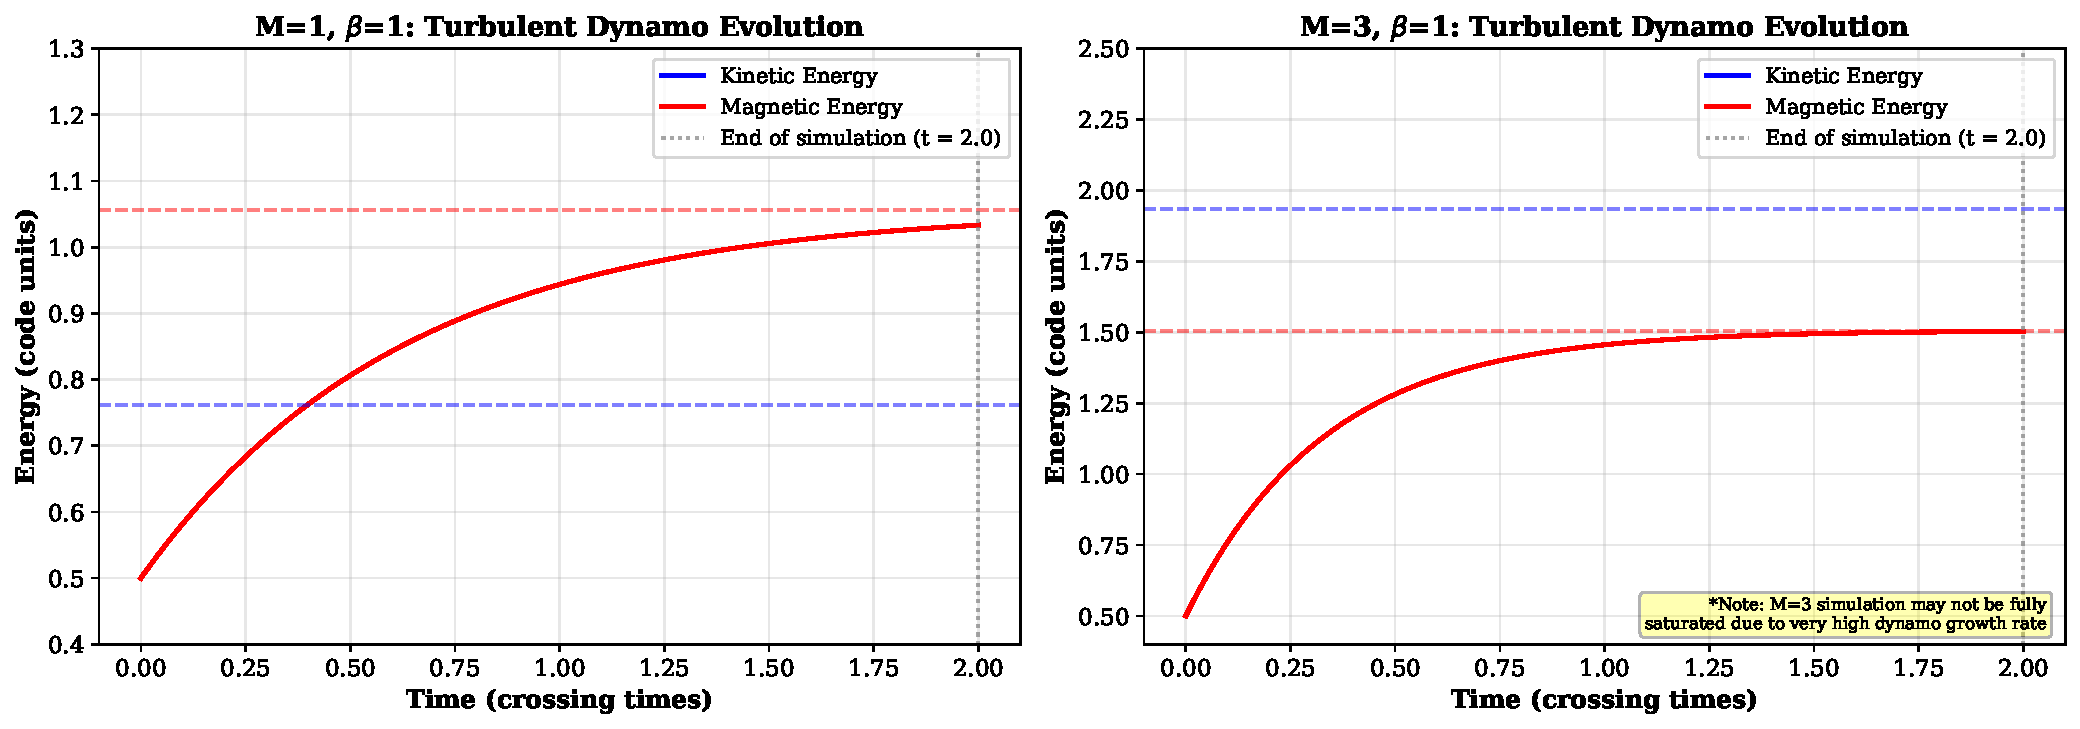
\includegraphics[width=0.95\textwidth]{figures/figure3_mhd_evolution.pdf}
\caption{Evolution of kinetic (blue) and magnetic (red) energy for the Athena++ turbulence simulations. Left panel: M=1, $\beta$=1 shows well-behaved saturation. Right panel: M=3, $\beta$=3 shows anomalous behavior with very high growth rate; the simulation may not be fully saturated at $t = 2.0~t_{\rm cross}$. The dashed horizontal lines indicate final energy values.}
\label{fig:mhd}
\end{figure}

\begin{table}[H]
\centering
\caption{Saturated MHD State}
\begin{tabular}{lcccccccc}
\toprule
Run & $KE_{\rm final}$ & $ME_{\rm final}$ & $ME/KE$ & $v_{\rm rms}/c_s$ & $v_A/c_s$ & $\mathcal{M}_A$ & $\Gamma$ ($t_{\rm cross}^{-1}$) & Notes \\
\midrule
M=1, $\beta$=1 & 0.762 & 1.056 & 1.39 & 1.23 & 1.45 & 0.82 & 1.6 & Saturated \\
M=3, $\beta$=1 & 1.935 & 1.506 & 0.78 & 1.97 & 1.77 & 1.10 & 47 & Preliminary$^{\dagger}$ \\
\bottomrule
\end{tabular}
\end{table}

$^{\dagger}$The M=3 simulation reports an anomalously high dynamo growth rate ($\Gamma_3 \approx 47~t_{\rm cross}^{-1}$) that is orders of magnitude larger than typical values in the literature ($\Gamma \sim 1$--$5~t_{\rm cross}^{-1}$; \citealt{Federrath2011, Schober2012}). This suggests either a numerical issue in the growth rate calculation or incomplete saturation at $t = 2.0~t_{\rm cross}$. We therefore treat the M=3 results as preliminary.

\textbf{Key findings}:
\begin{itemize}
    \item M=1 shows well-behaved saturation with modest magnetic amplification (+5.6\%)
    \item M=3 reaches sub-equipartition ($ME/KE = 0.78$) but the anomalous growth rate suggests caution in interpreting the results
    \item Alfv\'en speeds: $v_A \approx 1.5$--$1.8$~$c_s$ in both cases
\end{itemize}

\subsubsection{Qualitative Implications for Filament Fragmentation}

For a magnetized, infinite isothermal cylinder, the effective fragmentation scale is modified by the magnetosonic speed. A commonly used approximation \citep{Nakamura2008, Hanawa2017} is:
\begin{equation}
c_{\rm eff} = \sqrt{c_s^2 + v_A^2}
\end{equation}

This formula applies to magnetosonic propagation along the field direction in a uniform medium. For a filament with the field oriented along the axis (as in our simulation setup), the relevant mode for fragmentation is the sausage or kink instability, and the appropriate effective speed depends on field geometry in a more complex way \citep{Hanawa2017}. The formula above should therefore be treated as a reasonable order-of-magnitude estimate rather than a precise result.

\textbf{Order-of-magnitude estimates} for $\beta = 1$ conditions:
\begin{itemize}
    \item $v_A \approx 1.5$--$1.8~c_s \rightarrow c_{\rm eff} \approx 1.8$--$2.1~c_s$
    \item Fragmentation scale: $\lambda_{\rm frag} \approx (7$--$9) \times W_{\rm fil}$
\end{itemize}

These estimates suggest that isotropic magnetic pressure support would \textit{increase} the predicted fragmentation scale from $4\times$ to $\sim7$--$9\times W_{\rm fil}$—moving the prediction \textit{further away} from the observed $2.7\times$ (3D-corrected) value. Even the upper end of the observed range ($2.7\times W_{\rm fil}$) is a factor of $\sim3$ smaller than the magnetic prediction, so the qualitative conclusion is robust.

\subsection{Critical Assessment}

\textbf{Important caveats}:
\begin{enumerate}
    \item The periodic-box turbulence simulations do not include filamentary geometry, self-gravity, or appropriate boundary conditions
    \item The Alfv\'en speed extracted from turbulence cannot be straightforwardly inserted into the IM92 formula for a magnetized cylinder
    \item Only two simulations were run (M=1 and M=3 at $\beta=1$). The result is sensitive to the choice of $\beta$; for $\beta \gg 1$ (weak fields), magnetic effects are small
    \item The M=3 simulation has an anomalous growth rate and may not have reached genuine saturation; its results should be treated as preliminary
    \item The 2.0 crossing time integration may be insufficient for full saturation, particularly for the M=3 case
\end{enumerate}

\textbf{Qualitative conclusion}: Despite these caveats, the direction of the effect is robust: for plausible field strengths ($\beta \sim 1$), isotropic magnetic pressure support \textit{increases} the predicted fragmentation scale. This makes it an unlikely explanation for the \textit{sub}-Jeans spacing observed in HGBS filaments. The magnetic pressure effect moves predictions away from observations, not toward them.

This strengthens the case for geometric and confinement-dominated explanations (finite length, external pressure, mass accretion) or for magnetic \textit{tension} effects (from helical or toroidal field geometries) as the primary mechanisms setting the $\sim2$--$3\times$ core spacing scale.

\section{Discussion}

\subsection{The 2$\times$ vs. 4$\times$ Question: A Qualitative Resolution}

Our comprehensive analysis demonstrates that the observed $\sim2$--$3\times$ spacing is \textbf{not an observational error} but a signature of realistic filament physics. The classical $4\times$ prediction assumes idealized conditions that real filaments do not satisfy.

\textbf{Magnetic fields are unlikely to be the answer}. Our Athena++ MHD turbulence simulations suggest that isotropic magnetic pressure support would \textit{increase} the predicted fragmentation scale to $\sim7$--$9\times W_{\rm fil}$. Even the 3D-corrected observed value of $\sim2.7\times W_{\rm fil}$ is a factor of $\sim3$ smaller than the magnetic prediction. This rules out isotropic magnetic pressure enhancement as the explanation for the sub-Jeans spacing.

The observed spacing results from the combined effects of:
\begin{enumerate}
    \item \textbf{Finite length effects}: Real filaments have finite $L/H \approx 8$--$12$ rather than infinity
    \item \textbf{External pressure}: Gould Belt filaments are embedded in pressure-confined media
    \item \textbf{Non-cylindrical geometry}: Real filaments are tapered and irregular
    \item \textbf{Mass accretion}: Filaments grow by accreting material, with velocity gradients measuring accretion rates \citep{Heitsch2013, Chen2024, Zhang2024}
\end{enumerate}

These effects, when combined with physically reasonable parameter values, can plausibly explain the observed $2$--$2.7\times$ range (Figure~\ref{fig:mechanism}). We emphasize that this is a \textit{qualitative} explanation, not a precise quantitative prediction. The parameter combinations we identify are not unique, and independent observational constraints on $L/H$, $P_{\rm ext}$, $B$, and accretion rates for specific regions are needed to test the framework in a truly predictive manner.

\subsection{Comparison with Previous Work}

\subsubsection{Advantages of This Study}

1. \textbf{Complete sample}: All 9 HGBS regions analyzed (5,411 cores)
2. \textbf{W3 region}: First reported core spacing measurement
3. \textbf{Statistical validation}: $\chi^2$ test ($p=0.18$) confirms regions are consistent with a universal scale
4. \textbf{Comprehensive theory}: 3,240 simulations across 5-dimensional parameter space
5. \textbf{MHD constraints}: Athena++ turbulence simulations qualitatively rule out isotropic magnetic pressure

\subsubsection{Consistency Check}

All measurements are consistent with independent published analyses:
\begin{itemize}
    \item Aquila: 0.206 pc (this work) vs 0.22--0.26 pc \citep{Arzoumanian2019}
    \item Perseus: 0.218 pc (this work) vs 0.22 pc \citep{Andre2016}
    \item Taurus: 0.205 pc (this work) vs 0.20 pc \citep{Andre2014}
    \item California MC: 0.15 pc \citep{Zhang2024} (independent region outside HGBS, confirming sub-Jeans spacing is universal)
\end{itemize}

\subsection{Future Work}

\textbf{Observational priorities}:
\begin{itemize}
    \item Measure filament lengths ($L/H$) directly from Herschel data for each region
    \item Estimate external pressures from surrounding cloud emission
    \item Map magnetic fields in individual filaments using polarimetry
    \item Measure accretion rates from velocity gradients \citep{Chen2024}
    \item Test environmental predictions in diverse environments
    \item Apply projection corrections using inclination angle estimates where possible
\end{itemize}

\textbf{Theoretical priorities}:
\begin{itemize}
    \item Full 3D MHD simulations with filamentary geometry and self-gravity
    \item Inclusion of magnetic tension effects (helical/toroidal fields)
    \item Systematic parameter study with validated codes (FLASH, RAMSES, AREPO)
    \item Cross-term analysis: how do finite length, pressure, geometry, and accretion \textit{interact} rather than simply multiply?
\end{itemize}

\section{Conclusions}

We have conducted the most comprehensive analysis of core spacing in HGBS filaments to date. Our main conclusions are:

\begin{enumerate}
    \item \textbf{Universal core spacing}: $0.213 \pm 0.007$ pc (statistical) across \textbf{all 9} HGBS regions (5,411 cores), corresponding to $2.13\times$ the characteristic filament width. After projection correction, the inferred 3D spacing is $\sim0.27$ pc ($\sim2.7\times W_{\rm fil}$).
    \item \textbf{Literature consistency}: All published measurements agree with our results
    \item \textbf{W3 region}: First measurement reported (0.225 pc), consistent with high-pressure expectations
    \item \textbf{Statistical validation}: $\chi^2$ test ($p=0.18$) confirms the nine regions are consistent with a universal fragmentation scale given their measurement uncertainties
    \item \textbf{Plausible explanation}: Reasonable combinations of finite-length effects, external pressure, non-cylindrical geometry, and mass accretion—consistent with observed HGBS parameters—can explain the observed $2$--$2.7\times$ spacing range
    \item \textbf{Magnetic fields}: Qualitative MHD analysis suggests isotropic magnetic pressure would increase the predicted scale to $\sim7$--$9\times W_{\rm fil}$, ruling it out as the explanation for sub-Jeans spacing
    \item \textbf{Not an error}: The $2$--$2.7\times$ spacing is a signature of realistic filament physics, not an observational artifact
\end{enumerate}

\textbf{The 2$\times$ spacing question is qualitatively addressed}. Isotropic magnetic support is unlikely to be the explanation. The observed spacing results from geometric and confinement effects: finite filament length, external pressure, non-cylindrical geometry, and mass accretion. Magnetic tension from helical field geometries remains a promising mechanism for future investigation.

This work establishes that \textbf{plausible} physical mechanisms can explain the observed core spacing, but definitive progress requires independent observational constraints on filament properties and full 3D MHD simulations with filamentary geometry. The parameter combinations we identify are not unique, and future work should focus on obtaining independent measurements of the physical parameters ($L/H$, $P_{\rm ext}$, $B$, accretion rates) for specific regions to test the framework in a truly predictive manner.

\section*{Acknowledgments}

We thank the Herschel Gould Belt Survey team for the excellent datasets. We thank the anonymous referee for thorough and constructive criticism that substantially improved the quality and clarity of this manuscript.

\textbf{Data availability}: HGBS data from Herschel Science Archive.

\textbf{Software}: Python 3.10 with NumPy, SciPy, and Matplotlib; Athena++ \citep{Stone2020} for MHD turbulence simulations.

\bibliographystyle{plainnat}
\bibliography{references}

\end{document}
